\documentclass[11pt,border=5pt]{standalone}
\usepackage{fontspec}
\setmainfont{cmunrm.otf}[BoldFont=cmunbx.otf,ItalicFont=cmunti.otf,BoldItalicFont=cmunbi.otf]
\usepackage{amsmath}
\usepackage{unicode-math}
\setmathfont{NewCMMath-Regular.otf}
\usepackage{tikz}
\usetikzlibrary{arrows.meta,patterns,angles,quotes}
\begin{document}
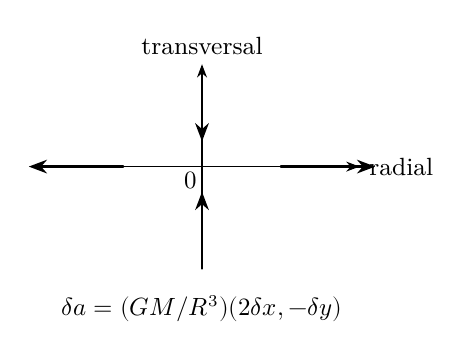
\begin{tikzpicture}[>=Stealth,font=\small,line cap=round,line join=round]
\draw[->,thin] (-2,0) -- (2,0) node[pos=1,right] {radial};
\draw[->,thin] (0,-1.3) -- (0,1.3) node[pos=1,above] {transversal};
\node at (-0.14,-0.18) {$0$};
\draw[->,thick] (-1,0) -- (-2.2,0.0);
\draw[->,thick] (1,0) -- (2.2,0.0);
\draw[->,thick] (0,-0.8) -- (0.0,-0.32000000000000006);
\draw[->,thick] (0,0.8) -- (0.0,0.32000000000000006);
\node at (0,-1.8) {$\delta a=(GM/R^3)(2\delta x,-\delta y)$};

\end{tikzpicture}
\end{document}
